\begin{frame}
  \frametitle{Por que EDEs?}
	\begin{empheq}[box={\Garybox[Cuantificación de Incertidumbre]}]{align*}
		EDO+ruido=Mejor \text{ } modelo
	\end{empheq}	
	\begin{overlayarea}{\textwidth}{.7\textheight}
		\begin{columns}
    		\column{.5\textwidth}
			\only<2-3>{		
			\begin{exampleblock}{Crecimiento de Poblaciones}
				$$
					\frac{dN}{dt}=a(t)N(t) \qquad N_0=N(0)=cte.
				$$
			\end{exampleblock}	
			}		
			\only<4-8>{	
			\begin{exampleblock}{Circuitos Eléctricos}
			\begin{align*}
				&L\cdot Q''(t)+
				R\cdot Q'(t)+
				\frac{1}{C}\cdot Q(t)
				=F(t)\\
				&Q(0)=Q_0\\
				&Q'(0)=I_0
			\end{align*}				
		\end{exampleblock}	
		}
		\column{.5\textwidth}
		\only<3>{
			\begin{empheq}[box=\shadowbox*]{equation*}		
				a(t)=r(t)+"ruido"
			\end{empheq}
		}	
		\only<5-7>{
			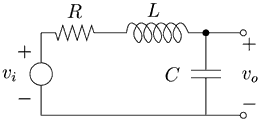
\includegraphics[width=\textwidth]{./images/CircuitRLC.png}		
		}		
		\only<6-7>{
		\begin{empheq}[box=\shadowbox*]{equation*}					
			F(t)=G(t)+"ruido"	
		\end{empheq}		
		}
	\end{columns}    
	\end{overlayarea}
\end{frame}
%%%%%%%%%%%%%%%%%%%%%%%%%%%%%%%%%%%%%%%%%%%%%%%
\begin{frame}
	\frametitle{Objetivo}
	\begin{alertblock}{Objetivo de la charla}
		\begin{itemize}
			\item<1> 
				\emph{Ilustrar} como formular modelos con EDEs perturbando un par\'ametro, 
			\item<2>
				Presentar las ideas de la aproximaci\'on de EDEs 
		\end{itemize}
	\end{alertblock}
\end{frame}
